\section{Robustness in the simulator}\label{sec:robust}

The real test fixes one workload, one burst size and one horizon; we varied each in the calibrated simulator (mixed batching). Each workload gets its own window $[1,\,hi]$ in multiples of its own $\lmiss$ ($hi$: the largest multiple at which all 10 from-empty runs stay stable) and is tested one third and two thirds of the way across it; a point passes if each arm meets its criterion in at least 7 of 10 seeds.

\begin{figure}[t]
\centering
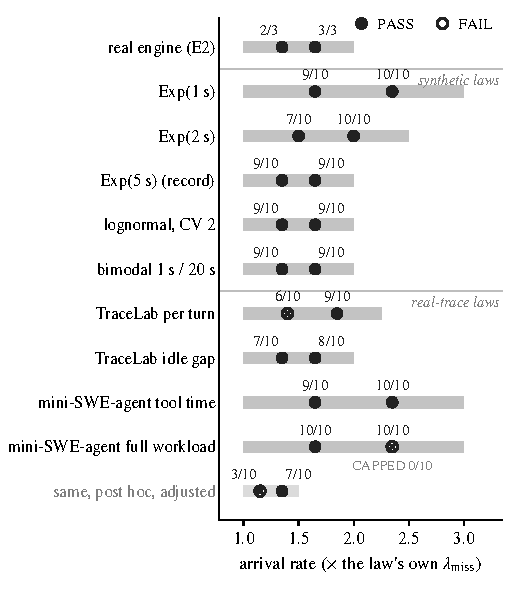
\includegraphics[width=0.94\columnwidth]{figs/fig5_robustness.pdf}
\caption{The paired test across tool-time laws (simulator). Gray bar: from-empty window $[1,\,hi]$ in multiples of each law's $\lmiss$. Markers: test points, filled = pass, crossed = fail (each arm in $\ge7$ of 10 seeds); number = BURST runs trapped of 10. Top row: the real engine (3 seeds, need 2). Bottom row: labelled post-hoc rerun of the mini-SWE-agent full workload.}\label{fig:robust}
\end{figure}

\paragraph{Tool-time laws.} With exponential tool times of mean 1, 2 and 5\,s, a lognormal law (mean 5\,s, coefficient of variation 2) and a bimodal law (80\% at 1\,s, 20\% at 20\,s), $\lmiss$ stays within 0.0718--0.0730\sps: it is a property of the server. Shorter tool times raise the peak ($\mu^*/\lmiss$ is 5.25, 4.57 and 2.97 for means of 1, 2 and 5\,s) and widen the window ($hi=3.0$, 2.5, 2.0); heavy tails at the same mean leave the edge at 2.0. The test passes at all 10 points (Fig.~\ref{fig:robust}): NOBURST and CAPPED succeed in 10 of 10 seeds everywhere, and BURST is trapped in 7 to 10 of 10.

\paragraph{Tool times from real agent traces.} We replaced the tool-time law by empirical tables from SyFI TraceLab, real sessions of two commercial coding agents used by 52 developers \todo{cite TraceLab, arXiv:2606.30560; not in refs.bib} (per-turn mean 8.51\,s with calls capped at 600\,s, median 0.237\,s, coefficient of variation 4.65; and an inter-request idle gap of mean 14.52\,s as an upper bound), and from mini-SWE-agent v2.0.0 on SWE-bench Verified~\citep{jimenez2024swebench} \todo{cite mini-SWE-agent; not in refs.bib} (mean 1.40\,s, median 0.104\,s, coefficient of variation 4.29). $\lmiss$ moved by $-0.8\%$ to $+1.3\%$. The peak moved to $n=32$ (TraceLab per turn) and 40 (idle gap), and a cap at the new peak recovered in 10 of 10 seeds. Eight of the 10 declared points passed, including the two exponential controls. The failure among the primary laws, TraceLab per turn at 1.40 $\lmiss$, is the slope rule: 6 of 10 BURST runs met it, all 10 were stuck at zero hits, and on 20 fresh seeds (post hoc) 17 met it. A secondary workload with mini-SWE-agent's own turn and token counts has sessions that outlive the declared measurement windows ($\lmiss$ is 0.0120\sps{} as declared, 0.0141 with a 20 times longer window); a labelled post-hoc rerun with longer horizons gives a narrower window, $[1,\,1.5]$, and a pass at 1.35.

\paragraph{Burst size and horizon.} At 1.35 and 1.65 $\lmiss$, a burst of 25 sessions never traps (0 of 10), 50 is a coin flip (5 and 6 of 10 trapped), and from 100 up every run is stuck below a hit fraction of 0.2. In runs extended to 30,000\,s after the burst, no trapped BURST run ever returned to a 100\,s window above a hit fraction of 0.5, all 20 ended with 468 to 1065 waiting requests, and no NOBURST run ever exceeded 50.

\paragraph{The slope rule is the fragile part.} Over the 100 BURST runs of the tool-time test the registered rule labels 90 trapped and 10 indeterminate, while all 100 are stuck at zero hits with an all-miss token rate. At 1.35 $\lmiss$ with 20 fresh seeds, 3 are indeterminate (Wilson interval $[0.05,\,0.36]$; median slope $0.77(\lambda-\lmiss)$ against a threshold of 0.5), so the real engine's one in three there is not surprising. Post hoc, a rule on the hit fraction alone would have called all six real BURST runs trapped; we report the registered rule.

\paragraph{The cap must follow the measured curve.} The right cap, 20 for the workload of record at 300k, moves to 32 or 40 with real tool-time laws and to 64--80 with the native pool; a cap above the new peak leaves $(\mu(N),\mu^*)$ open (Proposition~\ref{prop:cap}).
